\section{Idea}


Para la metaheurística de GRASP, tomaremos el algoritmo goloso previamente implementado y lo combinaremos con las diferentes búsquedas locales también previamente implementadas.

La idea es la siguiente, para cada paso del algoritmo, corremos una versión modificada del goloso de manera tal de permitir sierta aleatoriedad en los resultados. El algoritmo goloso será modificado de la siguiente manera:

\begin{algorithm}
  \begin{algorithmic}[1]\parskip=1mm
 \caption{ Goloso()}
 		\STATE{Numero los vértices de $1$ a $n$} 
		\STATE{Creo una cantidad $k$ de conjuntos donde iré guardando vértices}
 		\STATE{Para cada nodo $i$ de $1$ a $n$: }
		\STATE{\quad Para cada conjunto}
			\STATE{\quad\quad Sumo todos los pesos de las aristas de ($i$,$j$) con $j$ los vértices que están en el conjunto}
 		\STATE{\quad Del los mejores $x$ resultados, tomo uno al azar y pongo a $i$ en ese conjunto}
		\STATE{Devuelvo la respuesta}
\end{algorithmic}
\end{algorithm} 

Notar que si $x=1$ entonces estamos obteniendo el mismo algoritmo goloso que en el apartado anterior. En cambio, si tomo $x = k$ (esto es, tomo los $k$ mejores resultados, osea todos), estaría generando una solución complemtamente aleatoria. Cualquier solución en medio tomará una solución golosa, pero con sierto grado de aleatoriedad.

Luego a la solución obtenida por el algoritmo goloso modificado se le aplicarán una o varias de las búsquedas locales implementadas en un intento de mejorar aún mas la respuesta al óptimo.

Como primer criterio de corte el algoritmo se correrá un número finito de veces, que será determinado en el momento de experimentación.

Como segundo criterio de corte se realizarán estos mismos pasos hasta que luego de un número $x$ a determinar de intentos no haya sido posible mejorar la solución. En este punto se entrega la mejor respuesta obtenida hasta el momento.

Tras realizar diversas experimentaciones nos quedamos con dos versiones de GRASP, una que en el paso de búsqueda local usa la búsqueda local 2, y otra que en el paso de búsqueda local primero utiliza una búsqueda local 1 y luego una búsqueda local 3.

A continuación se formaliza de manera más precisa el algoritmo:

\begin{algorithm}
  	\begin{algorithmic}[1]\parskip=1mm
		 \caption{ GRASP1(SoluciónInicial) }
		 \STATE{while(true)}
		 	\STATE{\quad Corro el Algoritmo Goloso desarrollado previamente}
		 	\STATE{\quad Utilizo búsqueda local 2 para mejorar la solución obtenida previamente}
		 	\STATE{\quad Si conseguí una mejor solución que antes, la guardo}
		 	\STATE{\quad Si tras 1000 iteraciones no se pudo conseguir una mejor solución}
		 	\STATE{\quad\quad Devuelvo la solución}
	\end{algorithmic}
\end{algorithm}

\begin{algorithm}
  	\begin{algorithmic}[1]\parskip=1mm
		 \caption{ GRASP2(SoluciónInicial) }
		 \STATE{while(true)}
		 	\STATE{\quad Corro el Algoritmo Goloso desarrollado previamente}
		 	\STATE{\quad Utilizo búsqueda local 1 para mejorar la solución obtenida previamente}
		 	\STATE{\quad Utilizo búsqueda local 3 para mejorar la solución}
		 	\STATE{\quad Si conseguí una mejor solución que antes, la guardo}
		 	\STATE{\quad Si tras 1000 iteraciones no se pudo conseguir una mejor solución}
		 	\STATE{\quad\quad Devuelvo la mejor solución}
	\end{algorithmic}
\end{algorithm}

\section{Experimentación}

Ahora haremos una experimentación donde compararemos los tiempos de ejecución y los resultados del algoritmo de GRASP contra la solución exacta obtenida por backtracking.

Primero tomamos grafos de $25$ a $100$ nodos completos con aristas uniformemente distribuidas de $1$ a $100$ y analizamos los tiempos que dan los algoritmos:

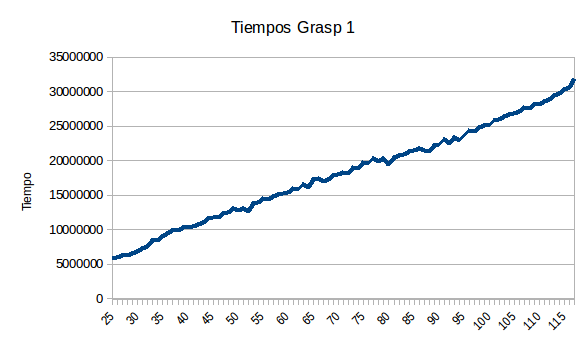
\includegraphics[scale=0.5]{Ej5/tiempog1.png}

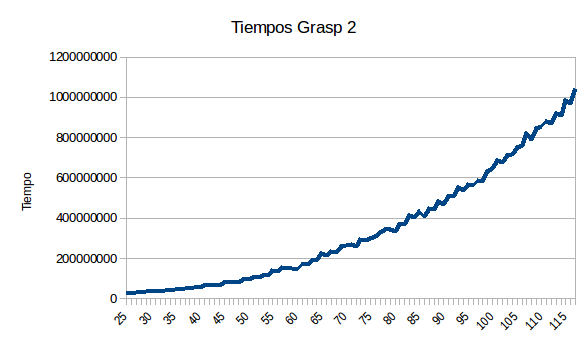
\includegraphics[scale=0.5]{Ej5/tiempog2.png}

Si bien se puede ver que no es exponencial, estas metaheurísticas dependen tanto de factores inherentes al algoritmo que se vuelve difícil de encontrar una complejidad de peor caso.

Además, se comparan como en los casos anteriores, las soluciones dadas por las dos heurísticas contra la solución exacta. La experimentación para este caso es igual a la realizada para el algoritmo goloso y para las búsquedas locales:

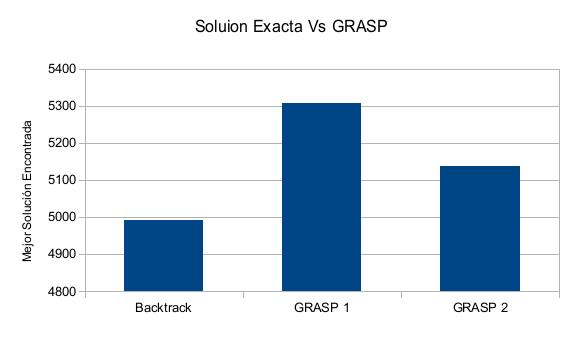
\includegraphics[scale=0.5]{Ej5/graspSol.jpg}

Puede verse aquí que la mejor de las heurísticas es la del GRASP 2, que no sólo encuentra soluciones más cercanas a la original, sino que en 17 de los 100 casos, logra encontrar la solución exacta. Esto, seguramente debido a que usa la búsqueda local 1, que como ya habíamos constatado en su experimentación, también lograba alcanzar soluciones exactas.

Finalmente, para los mismos casos de prueba antes vistos, también se miden los tiempos que tardan en encontrar la respuesta, obteniéndose los siguientes resultados:

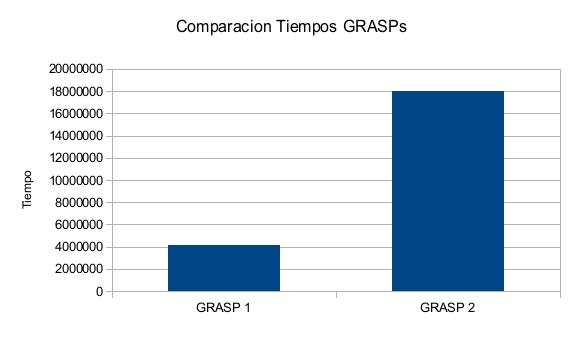
\includegraphics[scale=0.5]{Ej5/tiempos.jpg}

Puede verse que el hecho de encontrar soluciones exactas tiene su contrapartida en el hecho de que la metaheurística tarde significativamente más que la que no los encuentra.
